
Navigation data in satellite communication refers to the crucial information transmitted between satellites and ground-based receivers to facilitate accurate positioning and navigation. It includes data related to satellite orbits, precise timing, and other parameters necessary for determining the satellite's position relative to the Earth's surface.
\section{Frame structure}
NavIC master frame consists of $2400$ symbols, divided into $4$ subframes. Each subframe is $600$ symbols long. Each subframe has $16$ bit Sync word followed by $584$ bits of interleaved data. Subframes $1$ and $2$ transmit fixed primary navigation parameters. Subframe $3$ and $4$ transmit secondary navigation parameters in the form of messages. The master frame structure is shown in figure \ref{fig:master_frame}. 

\begin{figure}[ht]
\centering
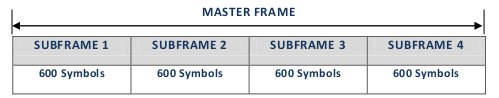
\includegraphics[width=0.8\columnwidth]{figs/master_frame.png}
\centering
\captionsetup{justification=centering}
\caption{Master Frame Structure}
\label{fig:master_frame}
\end{figure}

\noindent Each subframe is $292$ bits long without FEC encoding and sync word. It starts with TLM word of 8 bits and ends with $24$ bit Cyclic Redundancy Check(CRC) followed by $6$ tail bits. In subframes $1$ and $2$ navigation data is allotted with $232$ bits, starting from bit $31$. In subframe $3$ and $4$, $220$ bits are allotted starting from bit $37$. The typical structure of the subframes are shown in figure \ref{fig:frame_1_2} and figure \ref{fig:frame_3_4} respectively.

\begin{figure}[ht]
\centering
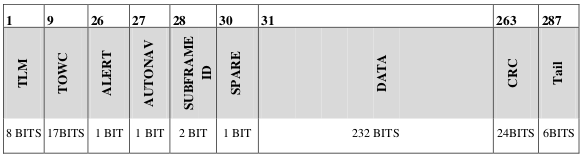
\includegraphics[width=0.8\columnwidth]{figs/1_2.png}
\centering
\captionsetup{justification=centering}
\caption{Structure of subframe 1 and 2}
\label{fig:frame_1_2}
\end{figure}

\begin{figure}[ht]
\centering
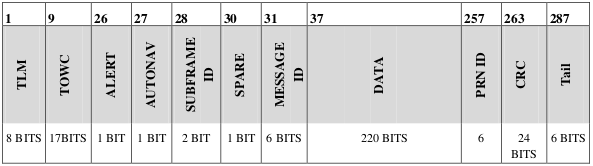
\includegraphics[width=0.8\columnwidth]{figs/3_4.png}
\centering
\captionsetup{justification=centering}
\caption{Structure of subframe 3 and 4}
\label{fig:frame_3_4}
\end{figure}

\section{Sync word and Tail bits}
Each subframe has a $16$ bit word synchronization pattern which is not encoded. Sync pattern is $EB90$ Hex. Tail bits consist of $6$ zero value bits added to the subframe and tail bits are part of FEC encoding. 

\section{Cyclic Redundancy Check(CRC)}
The parity coding of data signal follows $24$Q polynomial for each subframe. $24$ bits of CRC parity will provide protection against burst as well as random errors with undetected error probability of $2^{-24}$ for all channel bit error probabilities $0.5$.
\begin{equation}
    g(X) = \sum_{i = 0}^{24}g_{i}X^i\;\; 
\end{equation}

    $g_{i}=1$; for $i = 0,1,3,4,5,6,7,10,11,14,17,18,23,24$ \\
          = 0 otherwise

\let\cleardoublepage\clearpage
